\begin{landscape}
\begin{figure}
  \centering
  \begin{subfigure}[t]{0.6\textwidth}
    \centering
    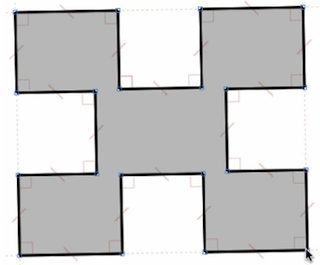
\includegraphics[width=0.8\linewidth]{img/jessica-constraint-example.png}
    \caption{initial state with 20 vertices, 20 line segments,
      and 45 low-level constraints. The user will move a corner, which
      violates many constraints. The following graphs illustrate error
      over thousands of constraint solving iterations.}
    \label{fig:jessica-initial}
  \end{subfigure}
  \hspace{0.03\textwidth}
  \begin{subfigure}[t]{0.6\textwidth}
    \centering
    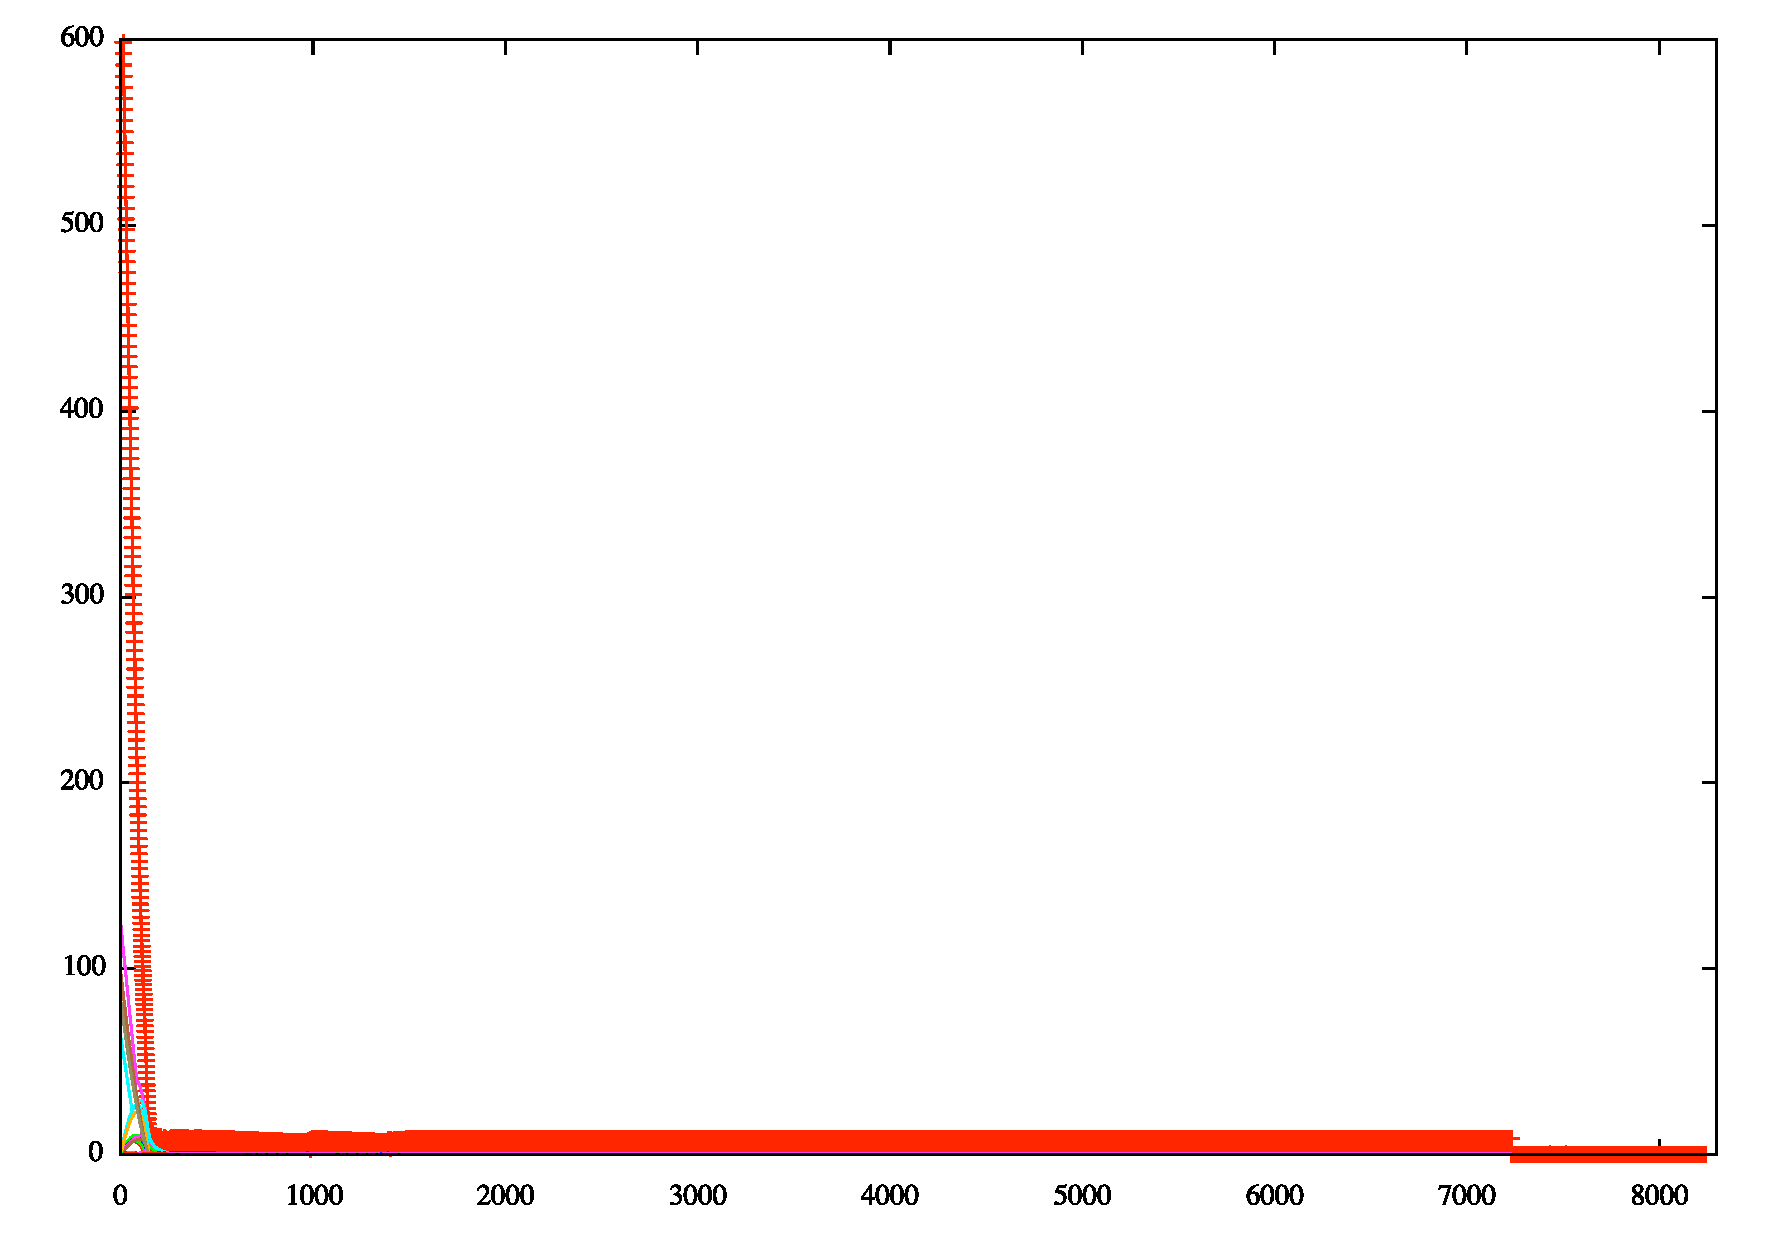
\includegraphics[width=0.8\linewidth]{img/jessica-norandom.pdf}
    \caption{Total error graph with weak randomness. It quickly comes
      close to a solution after 200 iterations, but does not fall
      below tolerance until after 8000 iterations.}
    \label{fig:jessica-norandom}
  \end{subfigure}

  \begin{subfigure}[t]{0.6\textwidth}
    \centering
    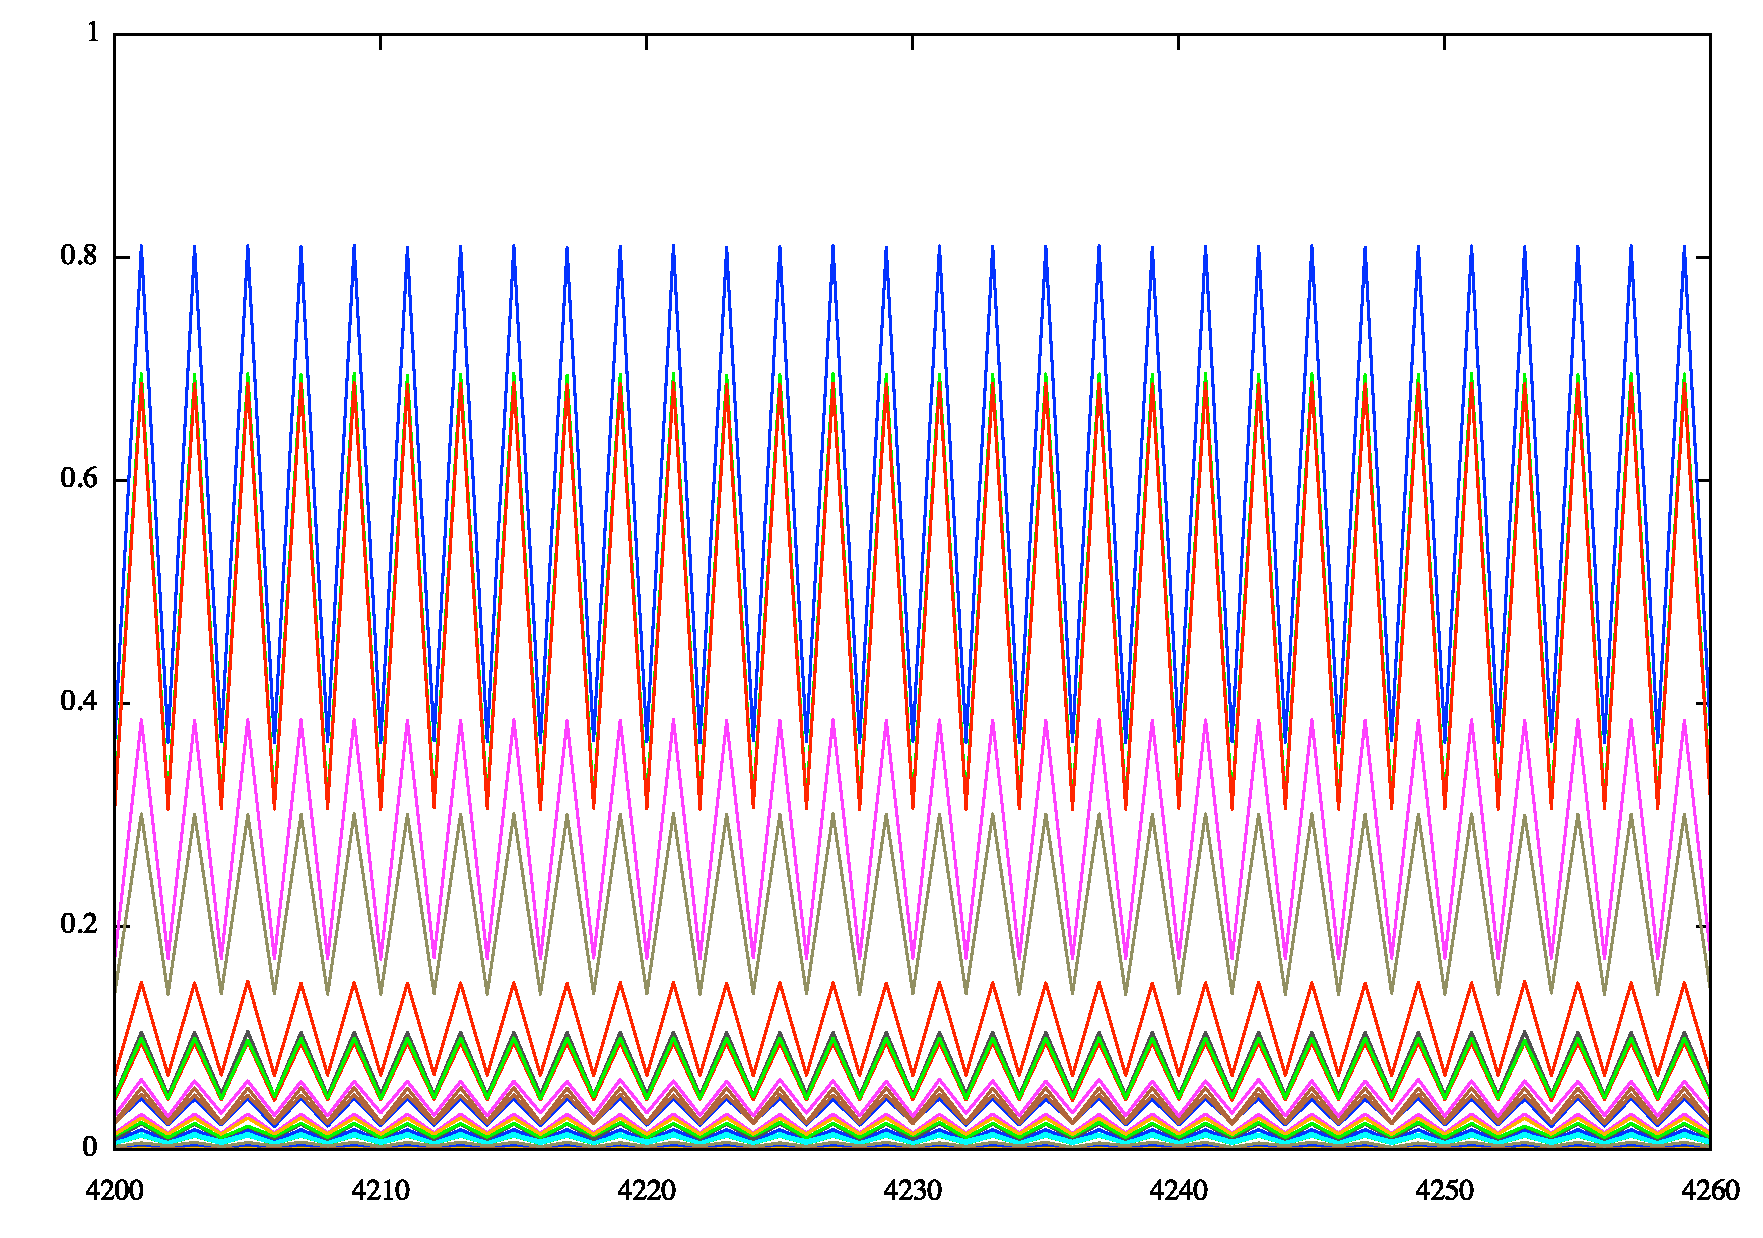
\includegraphics[width=0.8\linewidth]{img/jessica-norandom-closeup.pdf}
    \caption{Zoomed in portion of weak randomness
      Figure~\subref{fig:jessica-norandom}. States are `stuck'
      (iterations 4200 to 4260) oscillating between two states.}
    \label{fig:jessica-closeup}
  \end{subfigure}
  \hspace{0.03\textwidth}
  \begin{subfigure}[t]{0.6\textwidth}
    \centering
    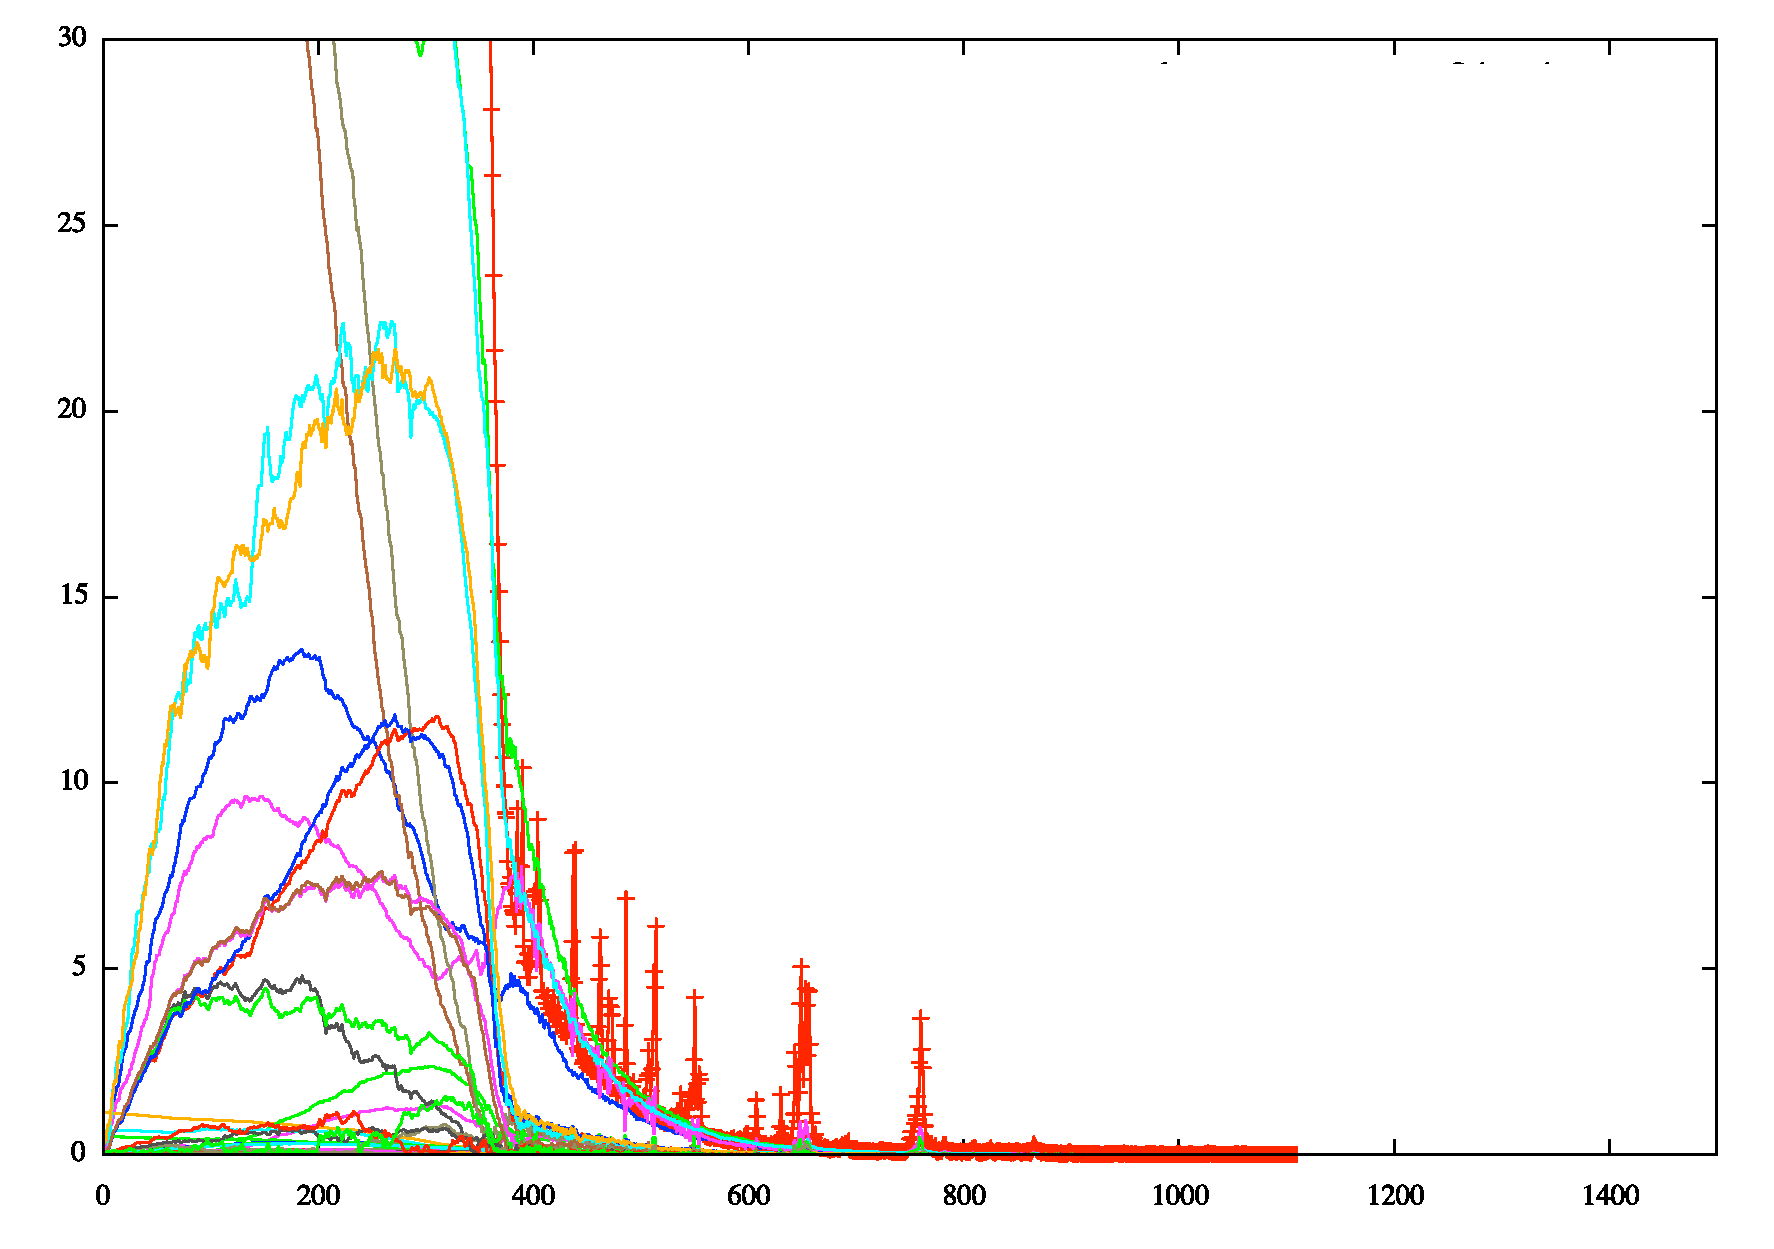
\includegraphics[width=0.8\linewidth]{img/jessica-with-fullrandom.pdf}
    \caption{Total error graph with full randomness converges below
      acceptable threshold after only 1100 iterations.}
    \label{fig:jessica-fullrandom}
  \end{subfigure}
  \caption[Constraint Solver Minimal vs. Full Randomness]{SIMI's
    constraint solver with minimal randomness
    (panels~\textit{\subref{fig:jessica-norandom}} and
    \textit{\subref{fig:jessica-closeup}}) compared with full
    randomness (panel~\textit{\subref{fig:jessica-fullrandom}}). In
    each graph, the red line at top is the total error. All other
    plots indicate error of individual low-level constraints.}
  \label{fig:jessica}
\end{figure}
\end{landscape}
